		\subsection{Metodología de las mediciones}
		
	Para calcular el aislamiento acústico provisto por el cuerpo de la pantalla se siguió el procedimiento de la Norma IRAM \texttt{4063-3/2002}: \textit{Acústica. Medición del aislamiento acústico en los edificios y de los elementos de construcción. Parte 3: Medición en laboratorio del aislamiento acústico a ruido aéreo de los elementos de construcción}.\\

	El ensayo se realiza en las cámaras de transmisión horizontal inferiores del laboratorio, que cumplen con los requerimientos de la norma IRAM \texttt{4063-1/2002}.\\
	
	En la Figura \ref{1_pantalla} se muestra cómo se colocaron las pantallas para realizar las mediciones:
	
		\begin{figure}[H]
			\centering
			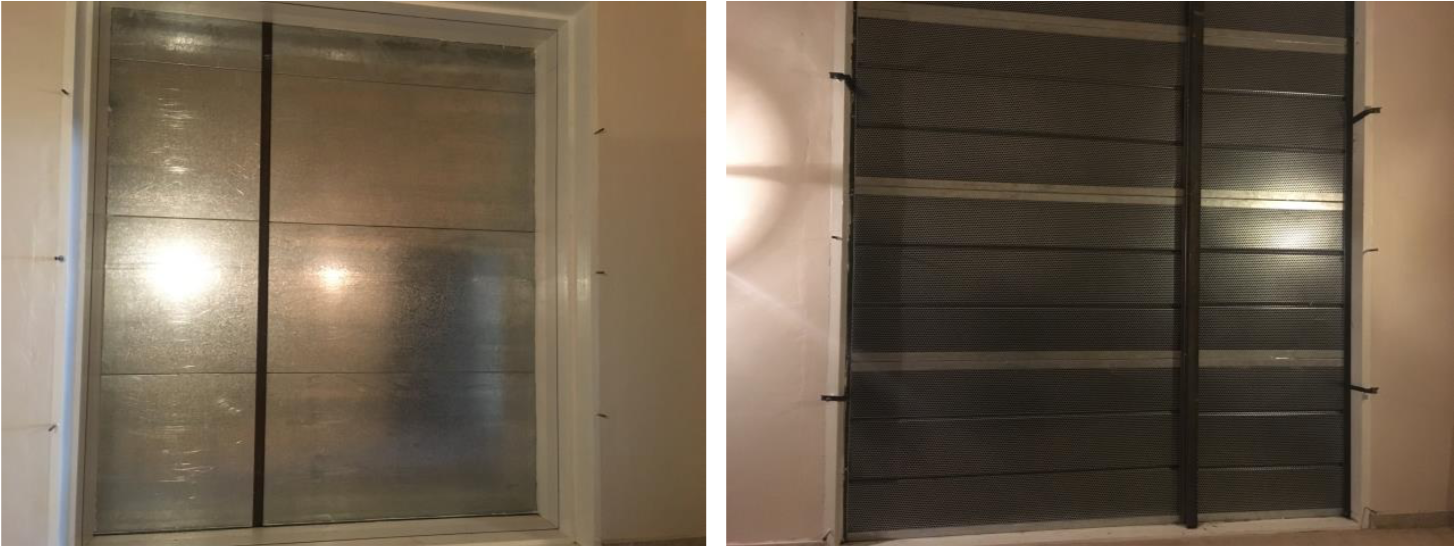
\includegraphics[scale=0.58]{1_pantalla.png}\\
			\caption{Montaje de pantalla para ensayo de aislamiento acústico.}
			\label{1_pantalla}
		\end{figure}
	
	La señal empleada para el ensayo es ruido de banda ancha. El proceso consiste en registrar, tanto en la sala emisora como en la sala receptora, el nivel sonoro continuo equivalente para las distintas frecuencias de ensayo. A los niveles sonoros medidos en el local receptor se les debe aplicar la corrección por ruido de fondo.\\
	
	Como resultado de este ensayo, se obtiene el \texttt{índice de reducción sonora R} de la muestra, expresado en decibeles. Dicho índice depende de la frecuencia, por lo que las mediciones se realizan en bandas de tercios de octavas, para las $18$ frecuencias centrales comprendidas entre \SI{100}{\Hz} y \SI{5000}{\Hz}.
	
	\subsection{Valores medidos}
	
	Se constató que la temperatura y la humedad permanecieron constantes durante el ensayo y los valores registrados fueron: \SI{20}{\celsius} y $52\%$, respectivamente. El volumen de las cámaras es de \SI{111.7}{\cubic\meter} (cámara emisora) y de \SI{113.9}{\cubic\meter} (cámara receptora). La muestra ensayada fue construida en el vano de \SI{10}{\square\meter} existente entre ambas cámaras.\\
	
	En la Tabla de la Figura \ref{1_mediciones} se presentan los valores de los parámetros medidos:
	
		\begin{figure}[H]
			\centering
			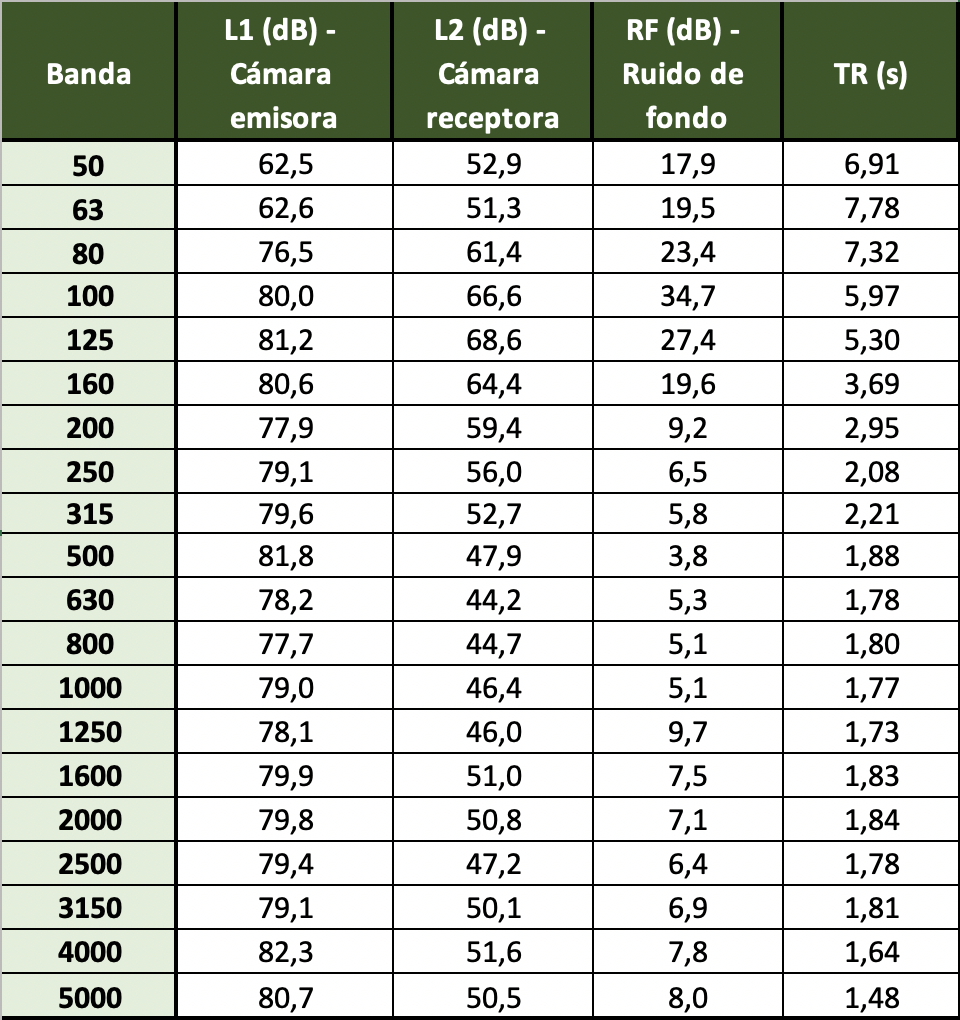
\includegraphics[scale=0.60]{1_mediciones.png}\\
			\caption{Niveles sonoros y tiempo de reverberación medidos.}
			\label{1_mediciones}
		\end{figure}
	
	\begin{itemize}
		\item \texttt{L1}: nivel sonoro continuo equivalente medido en cámara emisora, en dB;
		\item \texttt{L2}: nivel sonoro continuo equivalente medido en cámara receptora, en dB;
		\item \texttt{RF}: nivel sonoro continuo equivalente del ruido de fondo de la cámara receptora, en dB;
		\item \texttt{TR}: tiempo de reverberación medido en la cámara receptora, en segundos.
	\end{itemize}
	
	\subsection{Análisis de las mediciones}
	
		A partir de los datos de la tabla, se grafican los niveles sonoros en ambas cámaras para observar el comportamiento de las pantallas frente a distintas bandas de frecuencia:
	
		\begin{figure}[H]
			\centering
			\includegraphics[scale=0.70]{1_gráfico_nivel_sonoro.png}\\
			\caption{Nivel sonoro en la cámara emisora y receptore para cada banda de tercio de octava.}
			\label{1_gráfico_nivel_sonoro}
		\end{figure}
		
		Se puede ver cómo la presencia de las pantallas logra reducir el nivel sonoro en la cámara receptora frente al de la cámara emisora; el nivel de ruido de fondo en la cámara receptora no parecería afectar el nivel medido en ella. A frecuencias bajas, la pantalla reduce el nivel sonoro en un $15$ a $20$ \% para cada banda; luego de los $160$ Hz, comienza a aislar en mayor medida que lo que hacía para frecuencias menores, llegando a aislar el $40$ \% del nivel incidente.\\
	
		Con todos estos datos, se puede calcular el \texttt{índice de reducción sonora R} a partir de la siguiente expresión según la norma \texttt{4063-3}. que tiene en cuenta cada frecuencia y la temperatura al momento de la medición:
	
	\begin{equation}
		R = L1 - L2_{corregido} + 10\,log(\frac{S}{A_2})
	\end{equation}
	
	Este valor se calcula para cada banda de tercio de octava, ya que así se presentan los datos medidos de los niveles sonoros L1 y L2. El ruido de fondo medido en la cámara receptora sirve para poder realizarle una corrección al nivel sonoro medido en la misma con la fuente encendida y así poder calcular el índice R como se debe. En la cámara emisora es tanto más alto lo que se genera, que no tiene sentido corregir por ruido de fondo. El ruido de fondo se mide para cada frecuencia, y puede ocurrir que en algunas bandas el L2 no supere al ruido de fondo en la receptora. La corrección por ruido de fondo es un ejemplo típico de las restas energéticas; se realiza según la expresión:
	
	\begin{equation}
		L2_{corregido} = 10\,log(10^{0.1\,L2} - 10^{0.1\,RF})
	\end{equation}
	
	El parámetro S es la superficie de la muestra (\texttt{S = \SI{10}{\square\meter}}) y $A_2$ es el \texttt{área equivalente de absorción de la cámara receptora}:  
	
	\begin{equation}
		A_2 = 55.3\,\,\frac{V_2}{c\,\,TR_2}
	\end{equation}
	
	La velocidad del sonido varía con la temperatura según \texttt{c = 332 + 0.608\,T}. Usando el dato mencionado de \texttt{T = \SI{20}{\celsius}}, se calcula \texttt{c = \SI{344.16}{\meter/\second}}. \texttt{$V_2$} es el dato del volumen de la cámara receptora y \texttt{$TR_2$} es su correspondiente tiempo de reverberación para cada banda de frecuencias.\\

	Se hace el ensayo con filtros de tercios de octava (entonces va a haber 21 valores de cada variable que dependa de la frecuencia, que son: TR, L1, L2 y R).\\
	
	A continuación, se muestra la tabla de valores obtenidos con las expresiones anteriores para cada banda de frecuencia:
	
		\begin{figure}[H]
			\centering
			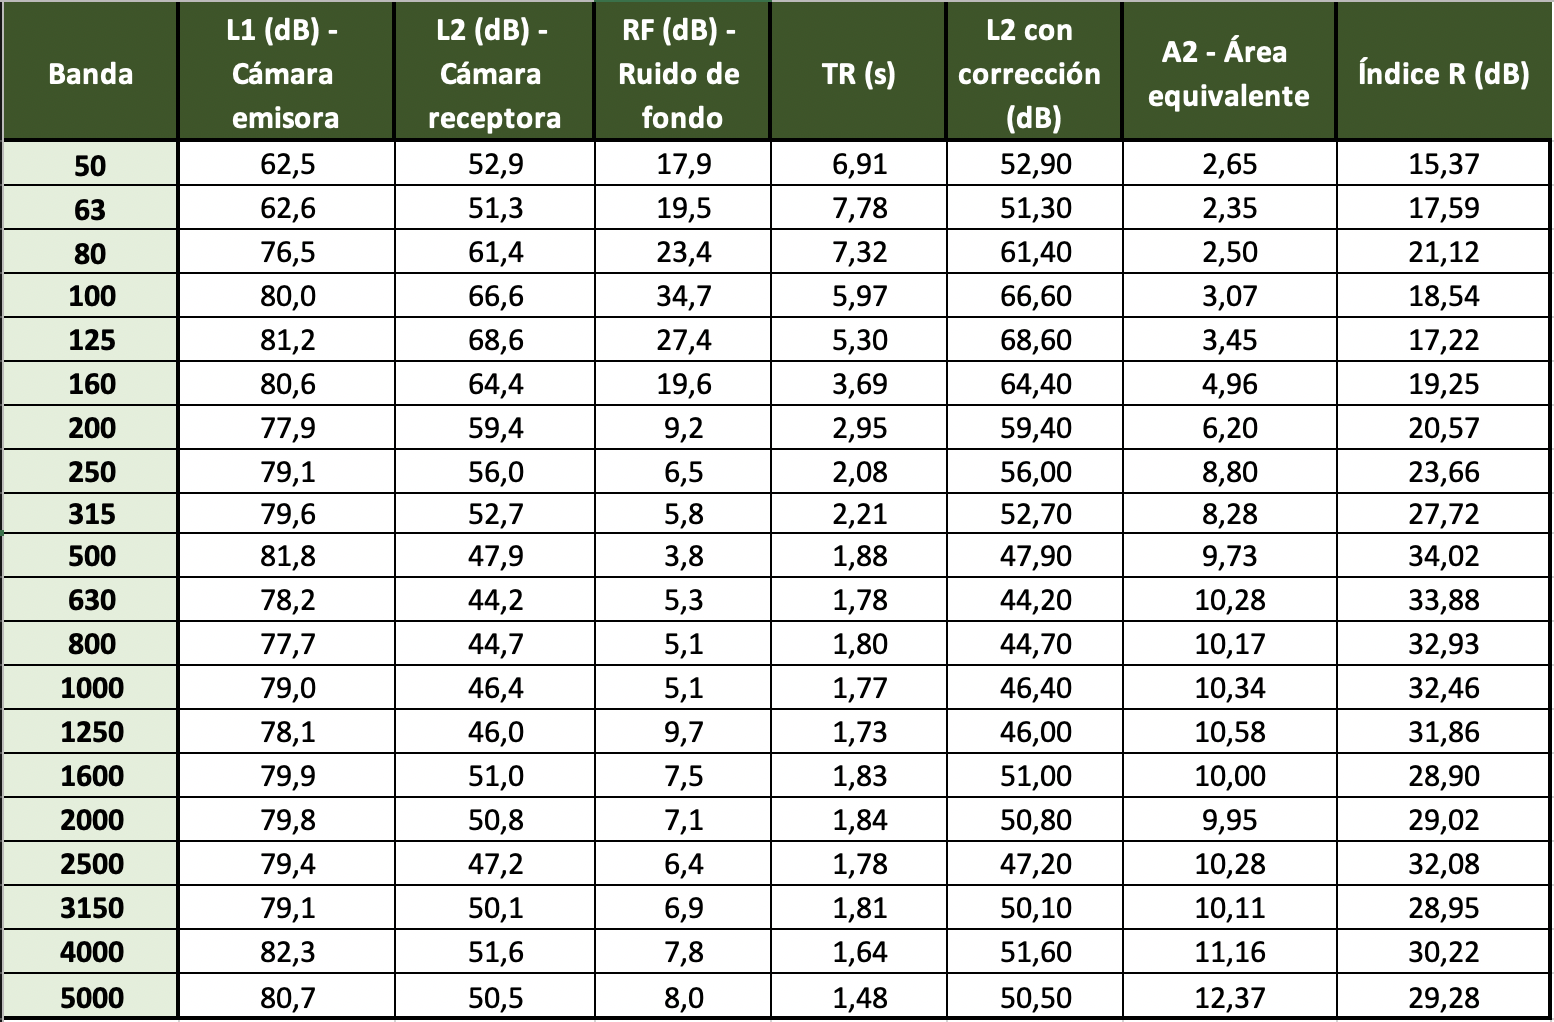
\includegraphics[scale=0.50]{1_tabla_final.png}\\
			\caption{Tabla de valores calculados para cada banda de frecuencia, para poder graficar el índice R.}
			\label{1_tabla_completa}
		\end{figure}
		
	Se observa que \texttt{$L2_{corregido}$} coincide con \texttt{L2} para todas las bandas de frecuencia; esto ocurre porque la diferencia entre el nivel \texttt{L2} y el ruido de fondo correspondiente es tan grande (al menos más de \texttt{10 dB} de diferencia para todos los casos), que el nivel no se ve afectado al realizar el desacople con la corrección. Con los datos de R que figuran en la Figura \ref{1_tabla_completa}, se grafica este índice en función de la frecuencia:
	
		\begin{figure}[H]
			\centering
			\includegraphics[scale=0.6]{1_gráfico_R.png}\\
			\caption{Gráfico del índice de reducción sonora para cada banda de frecuencias.}
			\label{1_gráfico_R}
		\end{figure}
		
		Mirando la curva de la Figura \ref{1_gráfico_R}, se puede ver cómo el índice R tiene un valor bajo para las frecuencias más bajas, y va aumentado su valor en cada banda, hasta llegar a un valor máximo de $34.02$ dB para los $500$ Hz. Luego de esa banda de frecuencia, baja un poco su valor, pero se sigue manteniendo en un nivel mayor al de las frecuencias bajas. Con este análisis, se puede decir que la pantalla aisla mejor para el rango de bandas entre los $500$ Hz t $5000$ Hz. Teniendo en cuenta que el ruido ferroviario tiene más componentes de altas frecuencias que el ruido de tráfico (debido al ruido de las ruedas del tren con el metal de las vías), este panel es más adecuado para instalar en el ambiente de vías ferroviarias que en una autopista.
	
	\subsection{Cálculo del índice de evaluación del aislamiento al ruido aéreo ($DL_R$)}
	
	A partir de los valores del aislamiento del sonido vía aérea dependientes de la frecuencia (índice R), y siguiendo los lineamientos de la norma \texttt{UNE-EN 1793-2}: \textit{Características intrínsecas relativas al aislamiento al ruido aéreo en condiciones de campo sonoro difuso}, se calcula el \texttt{número global}: este índice es calculado como la diferencia de niveles de presión sonora ponderados A, en decibeles, mediante la siguiente ecuación:
	
		\begin{equation}
			DL_R = -10\,log\left(\frac{\sum 10^{0.1\,L_i}\,10^{-0.1\,R_i}}{\sum 10^{0.1\,L_i}}\right)
		\end{equation}
	
		Donde:
		\begin{itemize}
			\item $R_i$: Índice de reducción sonora en la i-ésima banda de tercio de octava correspondiente a la muestra ensayada;
			\item $L_i$: Nivel de presión sonora de ruido normalizado ponderado A, en dB, de la i-ésima banda de tercio de octava del ruido normalizado que corresponda utilizar.
		\end{itemize}
		
		Se lo expresa en decibeles, y se redondea al entero más próximo.\\
		
		Para poder interpretar esta expresión, conviene expresarlo de otra manera, aprovechando las propiedades matemáticas del logaritmo y de la exponenciación:
		
		\begin{align}
			DL_R &= -10\,log\left(\frac{\sum 10^{0.1\,L_i}\,10^{-0.1\,R_i}}{\sum 10^{0.1\,L_i}}\right)\\
			DL_R &= 10\,log\left(\sum 10^{0.1\,L_i}\right) - 10\,log\left(\sum 10^{0.1\,(L_i - R_i)}\right)
		\end{align}
		
		De esta manera, se ve con mayor claridad que este índice refleja una resta energética entre el nivel de presión sonora de ruido normalizado ponderado A y el índice de reducción sonora R. La tabla del espectro normalizado ponderado A es un dato conocido que se puede ver en el Anexo.\\
		
		Teniendo en cuenta el espectro normalizado para el ruido ferroviario, se calcula siguiendo la expresión dada y se obtiene un valor de \texttt{$29.59 dB$}, que se debe redondear a:
		
		\begin{equation*}
			\boxed{DL_R = 30 dB}
		\end{equation*}
		
		Teniendo en cuenta el espectro normalizado para el ruido de tráfico, se calcula siguiendo la expresión dada y se obtiene un valor de \texttt{$28.07 dB$}, que se debe redondear a:
		
		\begin{equation*}
			\boxed{DL_R = 28 dB}
		\end{equation*}
	
		\subsection{Clasificación del comportamiento de aislamiento}
		
		De acuerdo con lo establecido en la norma citada, las categorías normalizadas en función de $DL_R$ son:
		
		\begin{table}[h!]
			\centering
			\begin{tabular}{cc}
			\toprule
			\textbf{Categoría} & \textbf{$DL_R$ (dB)}\\
			\midrule
			$B_0$ & No determinado\\
			$B_1$ & $DL_R$ < 15 \\
			$B_2$ & 15 a 24 \\
			$B_3$ & 25 a 34 \\
			$B_4$ & $DL_R$ > 34 \\
			\bottomrule
			\end{tabular}
		\end{table}
		
		Ambos valores obtenidos para el índice $DL_R$ se encuentran en la categoría \texttt{categoría B3}. Este resultado cumple con la especificación buscada para el aislamiento acústico.
